%!TEX root = ../template.tex
%%%%%%%%%%%%%%%%%%%%%%%%%%%%%%%%%%%%%%%%%%%%%%%%%%%%%%%%%%%%%%%%%%%%
%% chapter2.tex
%% NOVA thesis document file
%%
%% Chapter with the template manual
%%%%%%%%%%%%%%%%%%%%%%%%%%%%%%%%%%%%%%%%%%%%%%%%%%%%%%%%%%%%%%%%%%%%

The first (smaller) contribution of this thesis is an event-based framework called GO-Babel, available on \cite{goBabel}. This framework is a port in Golang \cite{golang} of Babel \cite{babel} with additions focused on fault detection and latency probing. Babel, in turn, is inspired on the model proposed by Yggdrasil \cite{akosThesis}.

The decision to build this framework arose from the need to use Babel for building the distributed protocols and the decision to use Golang during this dissertation (due to its primitives for building concurrent systems). Given that there was no implementation of Babel in Golang, and the current Babel implementation lacked some needed features such as a fault detector and a latency measurement tool, we implemented a new version in Golang with these additions.

\subsection{Overview}

In summary, this framework has the following main objectives:

\begin{enumerate}

    \item Abstract the networking layer, providing \textbf{channels}, which are essentially an abstraction over TCP connections, providing callbacks whenever outbound or inbound connections are established or terminated and whenever messages or sent or received from the respective operating system buffers.

    \item Execute protocols in a single-threaded environment and provide abstractions inter-protocol communications, such as request-reply and notification patterns.
    
    \item Provide abstractions for handling and managing time-based events (timers).

    \item Provide a layer of abstraction over node latency probing and fault detection.

\end{enumerate}

\begin{figure}[htbp]
    \centering
    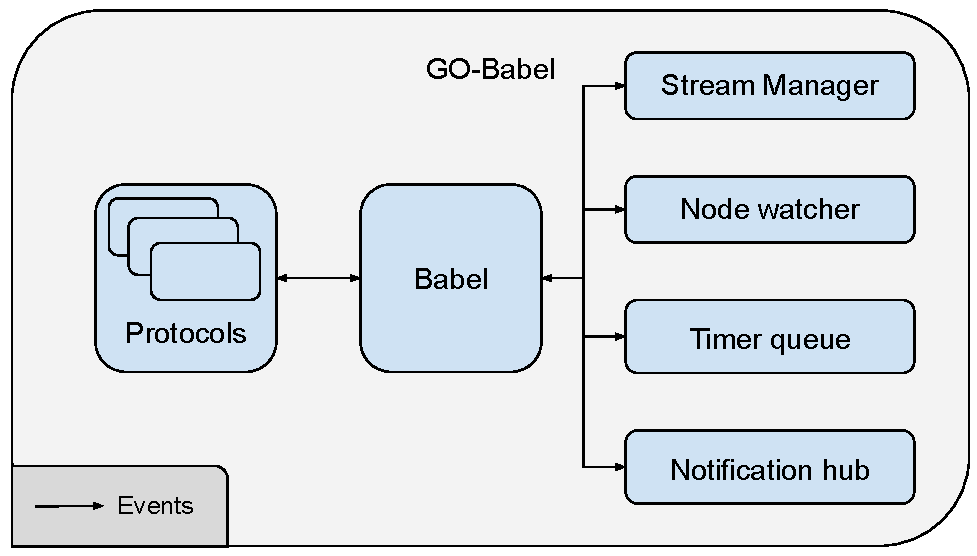
\includegraphics[width=\textwidth]{Chapters/Figures/Go-Babel-Overview.pdf}
    \caption{An overview of the architecture of GO-Babel}
    \label{fig:go-babel-overview}
\end{figure}

In Figure \ref{fig:go-babel-overview} we provide a high-level overview of the architecture of this framework, composed of five main components that communicate via callbacks. We now summarize each components' roles within the framework:

\begin{enumerate}

    \item Babel is the component tasked with initializing the protocols and all the other components according to issued configurations. It also acts as a mediator between the protocols and the remaining components.

    \item The Stream Manager is responsible for connecting to new peers, handling incoming/outbound connections, and sending messages through these connections. Interactions with this component are done through requests to, for example, dial a new node, or send a message through an established connection. When these requests are complete, the Stream Manager emits a notification back to the protocol that issued the request. The Stream Manager also provides operations for sending messages in temporary connections (either using TCP or UDP).

    \item The Timer Queue allows the creation and cancellation of timers and manages the lifecycle of timers issued by the protocols, delivering events to protocols whenever timers reach their expiry time. Two types of timers are allowed, the first are single-trigger timers, which only trigger once, and then are disposed of, the second type of timers periodic timers, which trigger at the set periodicity until cancelled.

    \item The Notification Hub is responsible for handling notifications and notification subscriptions, allowing protocols to substribe to certain notifications IDS. Any protocol subscribed to a notification ID always receives an event whenever another protocol emits that notification.

    \item The Node Watcher is the new addition to the framework. It allows for protocols to collect metrics regarding the latency and the current status (failed or running) of another node in the system. An explanation of this component in further detail is provided in the following section.

\end{enumerate}

As previously mentioned, the  Node Watcher is the only new addition to the framework, and consequently, it is the component explained in further detail. The remaining components of this framework were implemented similarly to the equivalent components of Babel \cite{babel} and Yggdrasil \cite{akosThesis}.

\subsection{Node Watcher} \label{sec:Node-Watcher}

The motivation to build this component was a lack of tools to measure latency in the original design of Babel. If, for example, a protocol were to measure the latency to a node without an active connection, it would need to establish a new TCP connection and use it to send the probes. In this case, both the fault detector and latency detector logic are in the protocol, which is sub-optimal since the same logic would have to be replicated by any protocol that wishes to optimize its active connections using latency as a heuristic. Alternatively, if a protocol measures latencies in a separate module asynchronously (making the code reusable), this would break the single-threaded nature of the execution of protocols in Babel (which impacts usability), and protocols would have to deal with race conditions of altering the state concurrently. Due to this, we believe that encapsulating this logic in an optional component and expose it in a Babel-compatible interface is the preferred option, which was the one used.

The Node Watcher is an optional component that, if registered, it will listen for probes in a custom port (specified in the configuration parameters) and send a reply with a copy of the contents back to the original senders. These probes are sent via UDP and carry a timestamp used by the original sender to calculate the round-trip time to the target node.

The main interface for the Node Watcher is composed of two functions, ``watch'' and ``unwatch''. When a node is ``watched'', the Node Watcher starts sending probes to the target node according to the issued configuration settings and instantiates a PHI-accrual fault detector \cite{phi-accrual-fd} together with a rolling-average latency calculator for that node.  When the node receives replies with copies of sent probes, it updates the corresponding rolling average calculator and fault detector. Conversely, when a node is ``unwatched'', the Node Watcher stops issuing the probes and deletes the fault detector and latency calculator.

When a protocol issues a command to watch a node, if the ``watched'' node fails to reply within a time frame, the Node Watcher falls back to TCP. This fallback aims to overcome cases where the watched node may be dropping UDP packets due to a constraint in its infrastructure (i.e., a firewall rule). If the watched node also does not accept the TCP connection, the Node Watcher sends a notification to the issuing protocol informing it failed to ``watch'' the node.

In order to prevent protocols from having to set timers to check the nodes' latency calculator or fault detector, the Node Watcher also allows the possibility of registering ``observer'' functions (or conditions), which return a boolean value based on the current node information. The Node Watcher then executes these functions periodically, and if one returns true, a notification gets sent to the issuing protocol. In order to prevent protocols from getting overloaded with notifications when a condition returns ``true'', these may configure a grace period, which the Node Watcher will wait for until re-evaluating the condition.

\subsection{Summary}

We believe Go-Babel is a small, yet valuable contribution to the distributed systems community. It not only as it provides more choice for developers in terms of choice of programming languages when choosing a distributed systems framework, but it also provides many abstractions which ease the development of self-improving protocols that employ latency as an optimization heuristic. Finally, it also offers a secondary fault detector which may be employed alongside the implicit fault detector granted by TCP connections. This is useful for cases when the TCP connection has failed yet the nodes did not receive any errors (e.g. when the ethernet cable is cut). Lastly, as the implementation is in Golang \cite{golang}, it allows easier integration with a range of packages already implemented in the language, many of which are useful for combining with GO-Babel. 
